%\documentclass[t,handout]{beamer}
\documentclass{beamer}
\listfiles

\mode<presentation>
{
  \usetheme[deutsch,titlepage0]{KIT}
% \usetheme[usefoot]{KIT}
% \usetheme{KIT}

%%  \usefonttheme{structurebold}\inputencoding{latin1}

  \setbeamercovered{transparent}

  %\setbeamertemplate{enumerate items}[circle]
  \setbeamertemplate{enumerate items}[ball]

}

\newcommand*{\JOKE}{}%

%\date{10.05.2010}
%\DateText

\newlength{\Ku}
\setlength{\Ku}{1.43375pt}

\usepackage[utf8]{inputenc}
\usepackage[TS1,T1]{fontenc}
\usepackage{array}
\usepackage{multicol}
\usepackage{listings}
\usepackage{amsmath}
\usepackage{alltt}
\usepackage{graphicx}
\usepackage{tabularx}
\usepackage{hyperref}
\hypersetup{
	pdftitle={PSE: Blockchain-basiertes E-Voting - Implementierung -Präsentation},%
	,%
}

\lstset{language=Java,
	basicstyle=\verysmall,
	keywordstyle=\color{blue}\ttfamily,
	stringstyle=\color{red}\ttfamily,
	commentstyle=\color{green}\ttfamily,
	morecomment=[l][\color{magenta}]{\#},
	breaklines=true,
	breakatwhitespace=true,
	tabsize=2
}
%\usenavigationsymbols
%\usenavigationsymbols[sfHhdb]
%\usenavigationsymbols[sfhHb]

\usepackage{pgf-pie}

\title[]{PSE: Blockchain-basiertes E-Voting - Qualitätssicherung}
\subtitle{Präsentation}

\author{Tim Fröhlich, Achim Kriso, Philipp Schaback, David Schuldes, Artem Vasilev\\ Phasenverantwortlicher: Achim Kriso}

\AuthorTitleSep{\relax}

\institute[]{KARLSRUHER INSTITUT FÜR TECHNOLOGIE (KIT)}

\TitleImage[width=\titleimagewd]{pictures/logo}

\begin{document}

\begin{frame}
\maketitle
\end{frame}

\begin{frame}
\frametitle{Überblick}
	\begin{itemize}
		\item Lösen \textbf{'aller'} Hyperledger-Fabric Probleme
		\item Wichtigsten UI-Fehler behoben
		\item[=>] \textbf{41} Issues closed
		\item Testumgebung für potentielle Weiterentwicklung
	\end{itemize}
\end{frame}

\begin{frame}
\frametitle{Aufwandseinteilung}
	\begin{figure}
		\centering
		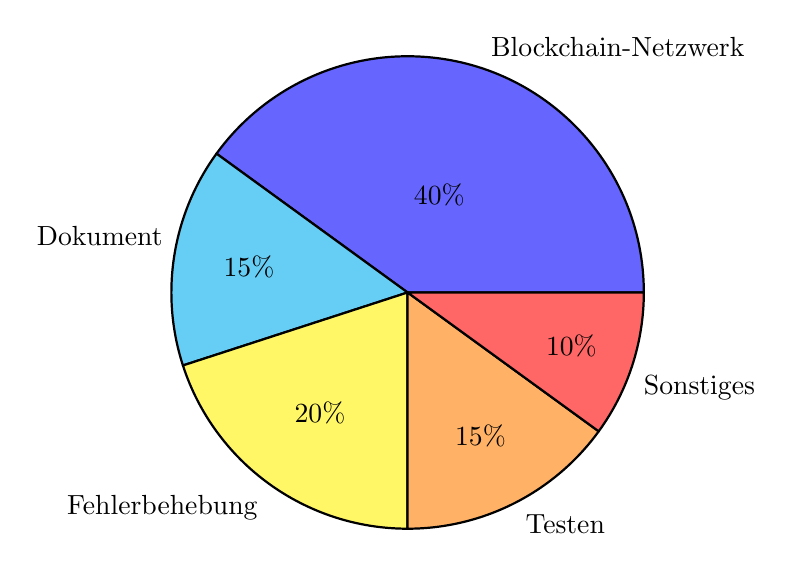
\begin{tikzpicture}
			\pie{40/Blockchain-Netzwerk, 15/Dokument, 20/Fehlerbehebung, 15/Testen, 10/Sonstiges}
		\end{tikzpicture}
	\end{figure}
\end{frame}

\begin{frame}
\frametitle{Rekonfiguration des Blockchain-Netzwerkes}
\framesubtitle{Ursprüngliches Problem}
	\begin{figure}
		\vspace{-5pt}
		\centering
		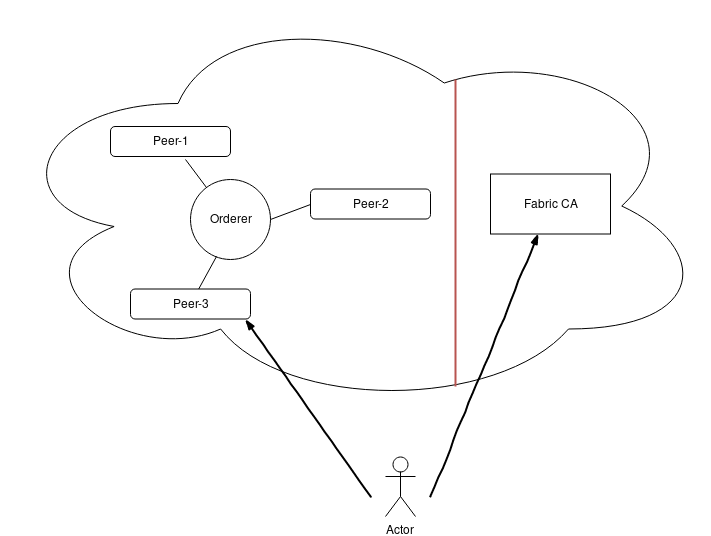
\includegraphics[width=\textheight]{pictures/wolkendiagramm}
	\end{figure}
	\begin{description}
		\item[Folge:] Alle Wähler hatten zusammen eine Stimme.
	\end{description}
\end{frame}

\begin{frame}
\frametitle{Rekonfiguration des Blockchain-Netzwerkes}
\framesubtitle{Lösung}
	\begin{itemize}
		\item Neue Konfiguration des Blockchain-Netzwerkes.
		\begin{itemize}
			\item Benutzung der richtigen Docker-Container (fabric-*-ca).
			\item Korrekte Kommunikation zwischen den einzelnen Peers und Oderer.
		\end{itemize}
	\end{itemize}
\end{frame}

\begin{frame}
\frametitle{Blockchain-Events}
	\begin{description}
		\item[Problem:] Events werden nicht vom Hyperledger-SDK empfangen.
		\item[Lösung:] Benutzen von Polling anstatt von Events.
	\end{description}
\end{frame}

\begin{frame}
\frametitle{Wechsel auf Polling}
	\begin{itemize}
		\item Entfernen des SDKEventListener Interface.
		\item Umschreiben des Hintergrund-Threads (\textcolor{green}{+}33 Zeilen, \textcolor{red}{-}36 Zeilen)
	\end{itemize}		
	\pause
	\begin{description}
		\item[Vorteil:] Unidirektionale Beziehung zwischen Statemanagement und SDKConnection.
		\item[Nachteil:] Größere Last auf das Blockchain-Netzwerk.
	\end{description}
\end{frame}

\begin{frame}
\frametitle{Testen der Software}
	\begin{itemize}
		\item Unit-Tests mithilfe von JUnit.
		\item Manuelle Tests für GUI.
	\end{itemize}
\end{frame}

\begin{frame}
\frametitle{Unit-Tests}
	\begin{itemize}
		\item Testen des Models und Control.
		\item Unit-Tests für die View weggelassen da unzuverlässig und nicht sehr aussagekräftig.
	\end{itemize}

	\pause
	\begin{block}{Code-Überdeckung}
		\begin{table}
			\begin{tabular}{l r r r}
				Paket & Linien \\
				\hline
				Model & 75\% \\
				Control & 48\% \\
			\end{tabular}
		\end{table}
	\end{block}
\end{frame}

\begin{frame}
\frametitle{Testplan}
	\begin{itemize}
		\item Eine Liste detaillierter Schritte mit Aktionen und erwarteten Reaktionen. \\
	\end{itemize}

	\begin{block}{Beispiel:}
		\begin{description}
			\item[\textbf{Aktion:}] Drücke die "Durchsuchen"-Schaltfläche.
			\item[\textbf{Reaktion:}] Datei-Auswahl-Menü erscheint.
		\end{description}
	\end{block}
	\begin{itemize}
		\item Insgesamt 40 Schritte.
		\item Testet:
		\begin{itemize}
			\item Wahl konfigurieren (inkl. Konfigurationsfehler)
			\item Wahl starten
			\item Wählen
			\item Wahlergebnis einsehen
			\item Import- und Export-Funktionalität
		\end{itemize}
	\end{itemize}
\end{frame}

\begin{frame}
\frametitle{Code-Überdeckung}
\begin{table}[h!]
	\begin{tabular}[t]{l r r r}
		Paket & Linien & Methoden & Klassen \\ 
		\hline
		Model & 89\% & 96\% & 100\% \\
		View & 82\% & 82\% & 90\% \\
		Control & 68\% & 87\% & 100\% \\ 
		\hline
		Total & 81\% & 82\% & 88\% \\
	\end{tabular}
\end{table}
\end{frame}

\begin{frame}
\frametitle{Performanz}
\framesubtitle{Erstellen einer Wahl, Export, Starten der Wahl und endgültiges Beenden}
	\textbf{Effektive Gesamtlaufzeit:} 7419 ms\\
	\textbf{Gesamter Speicherverbrauch:} 113 MiByte \\

	\pause
	\textbf{Speicherverbrauch:}
	\begin{table}[h!]
		\begin{tabular}[t]{l r r}
			Paket & Anteil & Größe \\ \hline
			org.hyperledger.* & 39\% & 44.170.288 Byte \\
			javax.imageio.ImageIO & 16\% & 15.789.784 Byte \\
			andere (nicht zuordenbar) & 45\% & 53.039.928 Byte \\
		\end{tabular}
	\end{table}

	\pause
	\textbf{Längste Methoden nach Ausführungszeit (mit Untermethoden):}
	\begin{table}[h!]
		\begin{tabular}[t]{lrr}
			Methode & Anteil & Zeit \\ \hline
			SupervisorSDKInterfaceImpl.createInstance() & 54\% & 4040 ms \\
			SupervisorSDKInterfaceImpl.registerUser() & 14\% & 1026 ms \\
			Andere (alle < 200 ms) & 32\% & 2353 ms
		\end{tabular}
	\end{table}
\end{frame}

\begin{frame}
\frametitle{Performanz}
\framesubtitle{Anmelden, Stimmabgabe bei einer laufenden Wahl}
	\textbf{Effektive Gesamtlaufzeit:} 4987 ms\\
	\textbf{Gesamter Speicherverbrauch:} 91 MiByte \\
	\pause
	
	\textbf{Speicherverbrauch:}
	\begin{table}[h!]
		\begin{tabular}[t]{l r r}
			Paket & Anteil & Größe \\ \hline
			org.hyperledger.* & 60\% & 54.621.125 Byte \\
			javax.imageio.ImageIO & 8\% & 7.281.324 Byte \\
			andere (nicht zuordenbar) & 32\% & 29.119.928 Byte \\
		\end{tabular}
	\end{table}

	\pause
	\textbf{Längste Methoden nach Ausführungszeit (mit Untermethoden):}
	\begin{table}[h!]
		\begin{tabular}[t]{l r r}
			Methode & Anteil & Zeit \\ \hline
			org.hyperledger.fabric.sdk.Channel.initialize() & 39\% & 1848 ms \\
			java.io.ObjectInputStream.readObject() & 19\% & 886 ms \\
			SDKInterfaceImpl.createHFClient() & 12\% & 558 ms \\
			Andere (alle < 400 ms) & 30\% & 1695 ms 
		\end{tabular}
	\end{table}
\end{frame}

\begin{frame}
\frametitle{Fazit}

\end{frame}


\begin{frame}
\frametitle{Ende}
\end{frame}

\end{document}